\documentclass[12pt]{article}

\usepackage[utf8]{inputenc}
\usepackage[T1]{fontenc}
\usepackage{amsmath,amssymb}
\usepackage{graphicx}
\usepackage{booktabs}
\usepackage{tabularx}
\usepackage[margin=1in]{geometry}
\usepackage{setspace}
\usepackage{fancyhdr}
\usepackage[hidelinks]{hyperref}
\usepackage{xurl}
\usepackage{caption}
\captionsetup{font=small,labelfont=bf,justification=raggedright,singlelinecheck=false}

\doublespacing
\setlength{\headheight}{14.5pt}
\pagestyle{fancy}\fancyhf{}\rhead{\thepage}\renewcommand{\headrulewidth}{0pt}
\graphicspath{{../figures/}}

\setlength{\parindent}{0.5in}
\setlength{\emergencystretch}{2em}
\newcommand{\ki}{k_i}
\newcommand{\kj}{k_j}

\begin{document}

% ===================== TITLE PAGE =====================
\thispagestyle{fancy}
\begin{center}
\vspace*{0.5in}
{\large\bfseries Dividing by a difference of noisy baselines:\\
why per-dyad estimates of a coupling parameter fail, and how to size a pooled alternative}

\vspace{0.5in}

Mark D. Izgarshev$^{1,*}$ and Sophie Noemi Kieckens$^{2,*}$

\vspace{0.25in}

$^{1}$Faculty of Economic Sciences, HSE University, Moscow, Russia\\
$^{2}$Scuola Svizzera di Roma, Rome, Italy

\vspace{0.15in}

$^{*}$These authors contributed equally to this work.

\vspace{0.75in}
\end{center}

\noindent\textbf{Corresponding author}\\
\mbox{}Mark D. Izgarshev\\
\mbox{}Faculty of Economic Sciences, HSE University\\
\mbox{}11 Pokrovsky Bulvar, Moscow 109028, Russia\\
Telephone: \mbox{+7 926 061 20 21}\\
E-mail: \mbox{markizgarsev90@gmail.com}

\vspace{0.15in}

\noindent\textbf{Co-author e-mail}\\
\mbox{}Sophie Noemi Kieckens: \mbox{funnyape67@gmail.com}

\vspace{0.25in}

\noindent\textbf{Word count:} approximately 9{,}000 (main text, excluding
abstract, references, tables and figure captions)

\vspace{0.25in}

\noindent\textbf{Keywords:} dyadic data; behavioural synchrony; convergence;
measurement error; actor--partner interdependence model; research design

\newpage

% ===================== ABSTRACT =====================
\begin{center}\textbf{Abstract}\end{center}
Studies of behavioural coupling (mimicry, synchrony, convergence) observe two
people together and compare them with baselines measured separately for each. A
per-dyad estimate of coupling therefore divides by a difference of two noisy
baselines. In a linear consensus model whose end-of-session observable is
$h(\theta)=(1-e^{-\theta})/\theta$, with $\theta=2\kappa T$, the precision of this
estimate is set by one combined signal-to-noise ratio $\zeta$: the interquartile
range of $\hat\theta$ is about $5.2/\zeta$. Discarding estimates outside $(0,1)$,
or selecting dyads on their own baselines, produces apparent coupling when none
exists, and a rank test on untruncated estimates, though valid, needs about three
times as many dyads as the pooled errors-in-variables estimator we propose, an
actor--partner model with replicate baselines and closed-form power. In
simulation its test held nominal size from 20 dyads per group and under several
departures from the model. Facilitation that differed between diners biased it,
and biased comparisons between groups when it differed between them; a test of
the partner effect was unaffected. In a public bite-event dataset, bites are
under-dispersed (variance/mean $\approx0.7$), and a single eating dyad would need
a meal of about six hours. A pooled comparison of two closeness groups needs
roughly 40 to 180 dyads per group if eating rates are stable traits. In the same
data, however, one person's meals differed as much as different people's, and at
the upper end of the stable spread the data allow, about 1,400 dyads per group
would be needed. Speech-rate convergence behaves similarly. Code is released as a
Python package.
\newpage

% ===================== INTRODUCTION =====================
\section*{Introduction}

A large class of studies asks whether two people become more alike when together.
Conversational partners converge on speech rate; interacting pairs align posture
and gaze; companions at a meal adjust their bite frequencies towards one another;
behaviour is mimicked more generally (Chartrand \& Bargh, 1999). The standard design
observes the pair jointly and compares what it sees against baselines measured
separately for each person, since without those baselines there is no way to say
whether an observed similarity reflects influence or pre-existing likeness.

When the coupling is estimated dyad by dyad, the design has a structural
weakness. The estimator must normalise the observed joint discrepancy by the
discrepancy expected from the two baselines alone, so its denominator is a
\emph{difference of two independently estimated baselines}. For two people who
behave similarly when alone, that difference is a small quantity known only up to
noise. Ratios of this kind have no finite moments (Hinkley, 1969; Marsaglia, 1965), they are
undefined when the denominator crosses zero, and analysis steps that look like
housekeeping, such as discarding estimates that fall outside the admissible
range, interact with the noise in ways that bias toward finding coupling.

This paper does four things. First, working in an explicit dynamical model of
within-meal coupling, we show that the precision of the per-dyad estimate is
governed by one combined signal-to-noise ratio. It joins the size of the
joint-session gap relative to its sampling variability and the size of the
baseline contrast relative to its standard error, and we calibrate the value it
must reach by simulation. Second, we show by simulation under no coupling that two
procedures the design invites manufacture coupling. Third, we give a pooled alternative. In
the slow-drive limit of the model, each diner's intake is a weighted combination
of their own and their partner's baseline rates, which is an actor--partner
interdependence model (Kenny et al., 2006) with one constraint. Estimating it
across dyads, with replicate solo sessions correcting for baseline measurement
error (Carroll et al., 2006; Fuller, 1987), never
divides by a single dyad's contrast, and its power has a closed form. We test it
against departures from the model that generated it: small samples, skewed rates,
a decaying drive, heterogeneous coupling and differential facilitation. Fourth, we
apply both analyses to two cases and release code that sizes a study and fits the
estimator.

The two cases were chosen to differ. The first is within-meal bite mimicry.
Companions adjust their bite frequencies towards one another (Bell et al., 2019;
Hermans et al., 2012; Sharps et al., 2015), people model one another's intake
(Bevelander et al., 2013; Cruwys et al., 2012; Vartanian et al., 2015), and
eating with familiar companions increases intake more than eating with strangers
(Clendenen et al., 1994; de Castro, 1994). The coupled models introduced below,
in which coupling acts as a restoring force on the intake gap, predict that the
gap between two diners' cumulative intakes contracts over the meal, and a public bite-event dataset (Kyritsis et al., 2019) lets every quantity in the calculation be estimated rather than assumed.
The second is speech-rate convergence, which has the same formal structure and
published variance components. In that literature, pooling has already succeeded:
Cohen Priva et al. (2017) detected convergence to the interlocutor's
baseline across a large telephone corpus by modelling baselines measured in other
conversations, and Cohen Priva and Sanker (2019) set out the limitations of difference-in-difference measures, which
compare the change in absolute distance between a speaker and an interlocutor. Our
analysis complements theirs. The index analysed here is a ratio, normalised by the
baseline contrast, rather than a difference, and we give a quantitative account of
when per-dyad estimation of a coupling parameter fails, together with a way to size
the pooled study in advance.

A conventional power analysis framed in numbers of dyads does not surface the
per-dyad problem, because it presumes the per-dyad estimate is well behaved. A
simulation-based power analysis matched to the estimator would surface it. The
diagnostics below can be read as such a simulation, reduced to formulas that can
be evaluated before any data are collected.

We are careful about scope. The analysis concerns designs that estimate a
coupling \emph{parameter} against individually measured baselines, which is what
testing the convergence predictions of a dynamical model requires. It does not
concern the short-window contingency measures used by the observational studies
that motivate those models. Hermans et al. (2012) operationalised mimicry as a
bite falling within a fixed five-second window after the partner's bite, across
70 dyads and 3{,}888 bites, using no solo baselines; Sharps et al. (2015) and Bell
et al. (2019) use comparable measures. Those designs estimate a different quantity
and are untouched by what follows. So are windowed cross-correlation and
cross-recurrence measures of synchrony, which describe the joint session without
dividing by a baseline contrast.

Our purpose is therefore prospective. We know of no published eating study that
estimates a coupling parameter dyad by dyad against solo baselines. The per-dyad
estimator analysed here is the one that a test of a dynamical model naturally
suggests, and the analysis is meant to inform such studies before they are run.
The statistical ingredients are standard: ratios of noisy quantities have no
moments (Hinkley, 1969; Marsaglia, 1965), Fieller intervals accommodate an
imprecise denominator (Fieller, 1954), selection on a noisy measurement produces
regression to the mean (Barnett et al., 2005), and replicate measurements correct
a regressor for measurement error (Fuller, 1987). What is specific to this paper
is their combination for this class of designs: the reduction of per-dyad
precision to a single ratio, the identification of the coupling as a constrained
actor--partner effect whose power has a closed form under replicate baselines,
calibrated inputs for two behaviours, and software that evaluates both before any
data are collected.

\section*{Two models of within-meal coupling}

Let $\ki(t)$ and $\kj(t)$ be the cumulative intakes of two diners, so that their
derivatives are bite frequencies, and let $D:=\kj-\ki$ be the intake gap. Intake
is counted in bites; $\beta$, $l$ and $\kappa$ carry units of $\mathrm{s}^{-1}$
and $A$ is dimensionless. Each diner has an individual drive $\beta e^{-lt}$ that
decays over the meal, a form standard in the cumulative-intake literature
(Kissileff et al., 1982; Thomas et al., 2017).

\subsection*{Intake matching}

The coupling must enter the two equations with opposite signs. A single positive
factor multiplying both diners' drives, in which company raises engagement for
both, cannot produce convergence: it divides out of the sign of the difference of
the two rates, so it sets how fast the gap moves but never which way, at any
magnitude and for any dependence on the state (Supplementary Section~S1). An
earlier dynamical model of within-meal mimicry (Kieckens \& Izgarshev, 2026) took
this form, with a shared affiliation factor that grows with the intake gap, and
that paper notes that the factor cannot steer the gap. We therefore write
\begin{equation}\label{eq:model}
\ki'(t)=A\,\beta_i e^{-l_i t}+\kappa\,D(t),
\qquad
\kj'(t)=A\,\beta_j e^{-l_j t}-\kappa\,D(t),
\end{equation}
in which the trailing diner is accelerated and the leading one slowed by an equal
amount. Here $\kappa\geq0$ increases with perceived closeness and $A\geq1$ carries
social facilitation, the robust finding that people eat more in company (Herman,
2015; Ruddock et al., 2019). Subtracting gives a linear
equation for the gap, $D'=\tilde g-2\kappa D$ with
$\tilde g(t)=A(\beta_j e^{-l_j t}-\beta_i e^{-l_i t})$, solvable in closed form
(Supplementary Section~S1).

Two features of \eqref{eq:model} are easy to over-read. Adding the two equations
cancels the coupling exactly, so with $\ki(0)=\kj(0)=0$ total intake is
independent of $\kappa$:
\begin{equation}\label{eq:conservation}
\ki(T)+\kj(T)=A\Bigl[\tfrac{\beta_i}{l_i}(1-e^{-l_iT})+\tfrac{\beta_j}{l_j}(1-e^{-l_jT})\Bigr].
\end{equation}
The consequence that both diners finish at the mean of their solo
intakes is therefore a property of the imposed antisymmetry, not an empirical
prediction of mimicry. Social facilitation is carried entirely by $A$, which is
logically independent of $\kappa$; empirically, facilitation acts mainly by
lengthening meals rather than by raising eating rate (de Castro, 1990; Feunekes et al., 1995; Pliner et al., 2006), and both
$A$ and $T$ cancel from the estimators below. Second, because the coupling
subtracts from the leading diner's rate, \eqref{eq:model} can in principle drive a
bite frequency negative. A sufficient condition for positivity is
$\kappa\geq\max(l_i,l_j)$ (Supplementary Section~S1). Across the 21 FIC meals,
maximum-likelihood fits (Method) gave a mean decay rate of $1.3\times10^{-4}\,\mathrm{s}^{-1}$, with a
95\% interval reaching $2.4\times10^{-4}\,\mathrm{s}^{-1}$, so in a 740-s meal the
condition holds for $\theta$ above about 0.2 to 0.4;
$\theta=1$ corresponds to $\kappa\approx6.8\times10^{-4}\,\mathrm{s}^{-1}$.

\subsection*{Rate matching}

The observations motivating this work concern rates, not cumulative amounts. The
corresponding rate model makes the frequencies state variables obeying a
consensus protocol with their own decay,
\begin{equation}\label{eq:ratemodel}
r_i'=-l_ir_i+\kappa(r_j-r_i),
\qquad
r_j'=-l_jr_j+\kappa(r_i-r_j),
\end{equation}
with $r_i(0)=A\beta_i$, $r_j(0)=A\beta_j$, and $\ki'=r_i$, $\kj'=r_j$. Setting
$\kappa=0$ recovers the individual drives exactly. Both eigenvalues are real and
negative, so $r_i,r_j\to0$ whatever the coupling. Two diners who both stop eating
have equal final rates whether or not they influenced one another, so end-of-meal
rate synchrony is uninformative. The positive quadrant is forward invariant, so
both frequencies remain non-negative with no parameter restriction (Supplementary
Section~S1).

\subsection*{Relation to consensus dynamics}

Both systems are two-agent linear consensus protocols with exogenous forcing, the
object studied in the opinion-dynamics and multi-agent literatures (Cucker \&
Smale, 2007; DeGroot, 1974; Hegselmann \& Krause, 2002; Olfati-Saber \& Murray,
2004; Ren \& Beard, 2008). We claim no novelty for the homogeneous analysis. What
is specific to eating is that the forcing, the individual drive, is integrable and
decays far more slowly than a meal lasts. The asymptotic regime that literature
studies is therefore the regime a meal never reaches, which is why the results
below are stated on a fixed horizon.

% ===================== METHOD =====================
\section*{Method}

\subsection*{What is estimable over a meal}

Fix a meal length $T$ and take $D(0)=0$. Define the \emph{contraction factor}
$\rho(T;\kappa)$ as the ratio of the intake gap at the end of the meal to the gap
the same two diners would show at $T$ with no coupling. Calibration (below) gives
$lT\ll1$ in most meals (the fitted decay rate sits at the optimiser's lower bound
in 13 of 21), so the individual drives are close to constant across a meal. In
that limit both couplings give the same contraction factor, and it does not
involve $l$:
\begin{equation}\label{eq:htheta}
\rho(T;\kappa)\;\longrightarrow\;h(\theta)=\frac{1-e^{-\theta}}{\theta},
\qquad \theta:=2\kappa T .
\end{equation}
$h$ is smooth and strictly decreasing on the whole real line, with $h(0)=1$ and
$h(\theta)\sim\theta^{-1}$ as $\theta\to\infty$ (Figure~1A; Supplementary
Section~S1). The parameter $\theta$ is the number of mimicry timescales elapsed in
a meal. Values $\theta<0$ give $h>1$ and correspond to divergence. The model
excludes them, but an estimator must be allowed to return them, for reasons
given below.

Two parameters cancel from the estimator. Combining \eqref{eq:htheta} with the
conservation identity \eqref{eq:conservation} in the same limit, and writing
$\Gamma:=\beta_j-\beta_i$ and $S:=\beta_i+\beta_j$ for the contrast and sum of the
two diners' solo rates,
\begin{equation}\label{eq:estimator}
h(\theta)=\frac{\kj(T)-\ki(T)}{\kj(T)+\ki(T)}\cdot\frac{S}{\Gamma}.
\end{equation}
The facilitation constant $A$, the meal duration $T$ and any absolute calibration
of the bite count cancel, leaving a ratio of an observed within-dyad asymmetry to
a solo contrast.

\subsection*{A ceiling on detectability across a closeness scale}

Suppose closeness, measured for example by the Inclusion of Other in the Self
scale (Aron et al., 1992), maps to coupling proportionally,
$\kappa=c\bar s$, with $\bar s$ ranging over a $q$-point scale,
$q=s_{\max}/s_{\min}$. The observable signal is the spread in the contraction
factor between the ends of the scale. Maximising over the position of the scale
gives, for the asymptotic factor,
\begin{equation}\label{eq:ceiling}
\Sigma^\star=\frac{\sqrt q-1}{\sqrt q+1},
\end{equation}
with the corresponding maximum for $h$ obtained numerically (Supplementary
Section~S1). For a seven-point scale these are 0.45 and 0.52: even under an
optimal design, a maximally and a minimally close dyad differ by about half a gap.
Equation~\eqref{eq:ceiling} assumes a ratio scale, under which a score of 7 means
seven times the coupling of a score of 1. The natural relaxation adds a baseline,
$\kappa=c(s_0+\bar s)$, under which \eqref{eq:ceiling} applies with
$q_{\mathrm{eff}}=(s_0+7)/(s_0+1)$. A baseline of one scale point costs a quarter
of the attainable spread, and a baseline of five reduces it to 0.20 (Table~1,
Figure~1B). The power calculations below compare $\theta=0$ with $\theta=1$, a
contrast in $h$ of 0.37 that lies inside this ceiling.

\subsection*{The per-dyad estimator and its precision}

Each quantity in \eqref{eq:estimator} is estimated with error. The joint-meal
counts are random even when the drives are known, with variance
$\phi\times$mean, where $\phi$ is the dispersion of the bite process ($\phi=1$
for a Poisson process, $\phi<1$ for a more regular one). A person's rate may also
differ from one meal to the next by more than counting noise. We write
$\sigma_o$ for this \emph{occasion} standard deviation, distinct from stable
differences between people. The sampling variance of the joint-session gap at
coupling $h$ is then
\begin{equation}\label{eq:gapvar}
\sigma_D^2=\phi A S T+2A^2h^2\sigma_o^2T^2 .
\end{equation}
This is sampling variability of the behaviour, not measurement error, and it
persists under perfect bite detection. The counting term grows as $T$ and the
occasion term as $T^2$. The baseline contrast, estimated from $m$ solo sessions of
length $T_s$ per person, has variance
$\sigma_{\hat\Gamma}^2=(\phi S/T_s+2\sigma_o^2)/m$.

To first order (Supplementary Section~S2), the variance of the per-dyad estimate
$\hat h$ from \eqref{eq:estimator} is
\begin{equation}\label{eq:zeta}
\mathrm{Var}(\hat h)\;\approx\;\frac{\sigma_D^2}{(A\Gamma T)^2}+\frac{h^2}{\nu^2}
\;=:\;\frac{1}{\zeta^2},
\qquad
\nu:=\frac{|\Gamma|}{\sigma_{\hat\Gamma}} .
\end{equation}
The first term is the inverse square of the gap signal-to-noise ratio,
$z_0=A\Gamma T/\sigma_D$ at $h=1$ when $\sigma_o=0$. The second involves the \emph{baseline contrast ratio} $\nu$, the number
of standard errors separating the two solo rates. We call $\zeta$ the combined
signal-to-noise ratio. With $\sigma_o=0$, $A=1$ and solo sessions as long as the
joint one, $\nu=\sqrt m\,z_0$, so $\zeta^{-2}=z_0^{-2}(1+h^2/m)$. The gap and the
baseline contrast are then one condition, not two, and once $m\geq4$ the
precision is set almost entirely by $z_0$.

Two properties of $\hat h$ govern how it should be used. It has no finite moments
at any $\nu$, because its denominator is a difference of estimates that can be
arbitrarily close to zero (Hinkley, 1969). What $\nu$ controls is the probability
that $\hat\Gamma$ has the wrong sign, $\Phi(-\nu)$: 2.3\% at $\nu=2$, 0.13\% at
$\nu=3$. And $\hat h$ can fall on either side of 1 by chance. Inverting it with $h$
extended to $\theta<0$ keeps the sampling distribution centred under the null.
Discarding estimates with $\hat h\geq1$, as a model that excludes divergence
might suggest, removes the half of the null distribution that points away from
coupling. Intervals should be Fieller intervals for the ratio (Fieller, 1954),
which remain valid when the denominator is imprecise; they can be unbounded,
which is informative.

\subsection*{A pooled estimator}

In the slow-drive limit, with $D(0)=0$, the end-of-meal intakes are
\begin{equation}\label{eq:apim}
\ki(T)=AT\Bigl[\tfrac{1+h}{2}\,\beta_i+\tfrac{1-h}{2}\,\beta_j\Bigr],
\qquad
\kj(T)=AT\Bigl[\tfrac{1+h}{2}\,\beta_j+\tfrac{1-h}{2}\,\beta_i\Bigr].
\end{equation}
This is an actor--partner interdependence model (Kenny et al., 2006) with actor
effect $(1+h)/2$ and partner effect $(1-h)/2$. The two sum to one by the
conservation property, and $h=(1-r)/(1+r)$ where $r$ is the partner-to-actor
ratio. The baselines $\beta$ are latent and are measured by the $m$ solo sessions.

For dyad $d$, let $y_d=\hat S_d(\kj-\ki)/(\kj+\ki)$, the observed asymmetry scaled
by the estimated baseline sum, which equals $h\Gamma_d$ plus noise with $A$ and $T$
cancelled. Let $x_d=\hat\Gamma_d$, the signed baseline contrast, and let $v_d$ be
its error variance estimated from the scatter of each person's solo sessions,
$v_d=(s_i^2+s_j^2)/m$. The pooled estimator is
\begin{equation}\label{eq:pooled}
\hat h_{\mathrm{pool}}=\frac{\sum_d y_d\,x_d}{\sum_d\bigl(x_d^2-v_d\bigr)} ,
\end{equation}
a method-of-moments errors-in-variables regression through the origin (Carroll
et al., 2006; Fuller, 1987). The labelling of $i$ and $j$ is arbitrary and the
estimator is invariant to it. It never divides by a single dyad's contrast;
dyads with small $|\Gamma_d|$ contribute little rather than contributing noise.
Its standard error comes from the M-estimation sandwich (Stefanski \& Boos, 2002).
Below about 50 dyads per group each dyad's score should be divided by $1-\ell_d$,
with leverage $\ell_d=(x_d^2-v_d)/\sum_d(x_d^2-v_d)$, the analogue of the HC3
correction for least squares (MacKinnon \& White, 1985); this kept the test at its
nominal size down to 20 dyads per group (Results). The corrected denominator
$\sum_d(x_d^2-v_d)$ must be clearly positive; if it is small relative to
$\sum_dx_d^2$, the sample carries too little true contrast and should be enlarged or
screened. The large-sample variance has a closed form (Supplementary Section~S4):
\begin{equation}\label{eq:pooledvar}
\mathrm{Var}(\hat h_{\mathrm{pool}})\approx
\frac{\sigma_e^2\bigl(\overline{\Gamma^2}+\sigma_u^2\bigr)+h^2\sigma_u^2\,\overline{\Gamma^2}
+h^2\sigma_u^4\bigl(2+\tfrac{1}{m-1}\bigr)}{n\,\bigl(\overline{\Gamma^2}\bigr)^2},
\end{equation}
with $\sigma_e^2=\phi S/(AT)+2h^2\sigma_o^2$ the noise in $y_d$,
$\sigma_u^2=\sigma_{\hat\Gamma}^2$, $\overline{\Gamma^2}$ the mean squared true
contrast across the $n$ dyads ($2\sigma_p^2$ for random pairing from a population
with between-person standard deviation $\sigma_p$), and $m\geq2$. Information now
accumulates as $1/\sqrt n$ whenever true contrasts vary at all.

Two alternatives were also evaluated. An instrumental-variable version replaces
$v_d$ by splitting each person's solo sessions in half and using one half's
contrast as an instrument for the other's. Ordinary least squares on the raw
baselines, $\sum y_dx_d/\sum x_d^2$, is attenuated by the reliability of
$\hat\Gamma$ (Fuller, 1987), and since attenuation pulls $\hat h$ below 1, it
reads as coupling.

The constraint that the actor and partner effects sum to one is what makes $A$
cancel. Without it, each diner's joint-session rate $k/T$ is regressed on their
own and their partner's baseline, with the same replicate correction for both,
the two diners of a dyad entering as two rows. The partner coefficient is then
$A(1-h)/2$. It is zero under $\kappa=0$ whenever a diner's facilitation depends
only on their own rate, whatever form that dependence takes (Supplementary
Section~S8). Its size depends on $A$, so it does not estimate $h$, but its test of
$\kappa=0$ needs neither equal facilitation nor a comparison group. Its standard
error comes from a delete-one-dyad jackknife.

Closeness groups made of friends or couples cannot be paired at random or
screened, and partners' rates may be alike. If partners' stable rates have
correlation $\rho$, the mean squared contrast falls to $2\sigma_p^2(1-\rho)$, which
enters \eqref{eq:pooledvar} directly.

\subsection*{Simulation studies}

All simulations used the slow-drive form \eqref{eq:apim}. Each person had a stable
mean rate $\beta_p$; on any one occasion their rate was $\beta_p+\varepsilon$ with
$\varepsilon\sim N(0,\sigma_o^2)$; counts were drawn with variance $\phi$ times
their mean (discretised normal; $\phi=0.7$, below). Parameters were set from the
FIC calibration: mean rate $0.0867\,\mathrm{s}^{-1}$ per person, solo sessions of
740\,s, and a between-meal standard deviation of rates of
$0.0130\,\mathrm{s}^{-1}$, split between stable ($\sigma_p$) and occasion
($\sigma_o$) components in the proportions stated.

\emph{Per-dyad.} For each cell we drew 6{,}000 dyads at fixed contrast
$\Gamma\in\{0.0124,\allowbreak 0.025,\allowbreak 0.0375,\allowbreak 0.05\}\,\mathrm{s}^{-1}$, meal length
$T\in\{740, 1500, 3000\}$\,s, $m\in\{1,\allowbreak2,\allowbreak4,\allowbreak8,\allowbreak16,\allowbreak64\}$ solo sessions of length $T$,
and $\theta\in\{0,1\}$. Varying $m$ at fixed $\Gamma$ and $T$ changes $\nu$ while
holding $z_0$ fixed, which separates the two. We formed $\hat h$, inverted it over
the whole real line, with $\hat\theta=+\infty$ when $\hat h\leq0$, and recorded the
median and interquartile range (IQR) of $\hat\theta$ and the coverage of 95\%
Fieller and delta-method intervals. We also reproduced two practices that the
design invites:
retaining only estimates with $0<\hat h<1$, and retaining only dyads whose
estimated contrast ratio $\hat\nu$ exceeded 2 or 3. Further cells added occasion
variance. Finally, two groups of 50 to 400 randomly paired dyads ($\theta=0$ and
$\theta=1$, or $\theta=0$ in both; 12-minute meals; $m=4$; all variation stable or
half occasional) were compared with a Mann--Whitney test on the untruncated
estimates.

\emph{Pooled.} Two groups of $n\in\{50,100,200,400\}$ dyads, with $\theta=0$ and
$\theta=1$ (power) or $\theta=0$ in both (size), were crossed with
$T\in\{740,1500,3000\}$\,s, $m\in\{2,4,8\}$ solo sessions of 740\,s, occasion
share $\sigma_o^2/(\sigma_o^2+\sigma_p^2)\in\{0,0.5\}$, and two pairing schemes.
The schemes were random pairing, and pairing opposite terciles of a single,
independent screening meal per candidate. Each cell had 2{,}000 replicates (1{,}000
for $n\geq200$). The test was a two-sided $z$-test on the difference of the two
group estimates with sandwich standard errors.

\emph{Robustness.} A further set of simulations departed from the assumptions of
\eqref{eq:pooledvar}, at 12-minute meals, $m=4$ and 100 dyads per group unless
stated, with 4{,}000 replicates per cell and the leverage-corrected standard error:
(R1) 20 and 30 dyads per group; (R2) lognormal stable rates and centred gamma
occasion effects (shape 2) with the means and variances used above; (R3) joint and
solo sessions generated from the full intake-matching model \eqref{eq:model}, each
person's decay rate drawn uniformly on $[0,l_{\max}]$, including joint sessions
longer than the solo sessions; (R4) dyad-specific coupling,
$\theta_d\sim\mathrm{Gamma}(2,0.5)$, with mean 1; and (R5) facilitation that differs
between diners, $A_p=1.1\,(1+\delta z_p)$ with $z_p$ the standardised solo rate and
$\delta=\pm0.05$; (R6) the same facilitation in one group only, with the
partner-effect test alongside; and (R7) one group of pre-existing pairs whose
stable rates had correlation 0.3 or 0.6, with coupling that was constant or that
fell with the pair's contrast. Details are in Supplementary Sections~S7 and S8.

\subsection*{Dataset and calibration}

Model parameters were estimated from the Food Intake Cycle (FIC) dataset (Kyritsis
et al., 2017, 2019), which provides frame-accurate ground-truth bite start times for 21
meal sessions from 12 participants eating individually in a cafeteria, each
choosing their own food. We take a meal's length $T$ to be the time from the
start of its recording to the end of the last bite (mean 738\,s, median 743\,s).
The first bite came on average 34\,s after the recording began; from first to last
bite, meals lasted 699\,s on average, close to the 704\,s the dataset reports. FIC was
chosen over two alternatives. The Clemson Cafeteria dataset distributes derived
bite counts rather than timestamped events, and OREBA records participants eating
in groups, which would contaminate solo baselines with the coupling under study.
FIC's bite annotations are human ground truth, so detection error does not enter.

\emph{Drive.} A two-parameter non-homogeneous Poisson model,
$\lambda(t)=\beta e^{-lt}$, was fitted to each meal by maximum likelihood, with $l$
searched between $10^{-7}$ and $1\,\mathrm{s}^{-1}$. Its
only role here is to show that $l$ is not identified at meal length: 13 of 21
meals put $l$ at the lower bound, as did least-squares fits to the cumulative
curve (also 13 of 21, at a lower bound of $10^{-6}\,\mathrm{s}^{-1}$). In a holdout
comparison, the saturating exponential, a constant rate, a straight line, the
quadratic of Kissileff et al. (1982) and the logistic model of Thomas et al. (2017)
were fitted by least squares to the cumulative curves of 17 meals, and their mean
parameters predicted the other four. Scored on bites counted in consecutive 60-s
windows, every model had a negative $R^2$ ($-0.03$ to $-1.60$), as it did when each
meal was predicted from the other 20 ($-0.02$ to $-1.03$).
 In the slow-drive limit the drive is the mean rate, which we estimate by
$N/T$ with sampling standard error $\sqrt{\phi N}/T$. The standard error of
$\beta$ from the two-parameter fit should not be used as the precision of a solo
baseline: it is inflated by the near-unidentified $l$ with which $\beta$ trades
off, and so understates how distinguishable solo rates are (see Results).

\emph{Dispersion.} We estimated $\phi$ two ways: from the variance-to-mean ratio
of bite counts in consecutive windows of 20 to 180\,s within each meal, pooled
across meals, and from the squared coefficient of variation of inter-bite
intervals, which equals the long-window Fano factor of a renewal process (Cox,
1962). A bootstrap over meals gave the interval.

\emph{Variance components.} The between-meal variance of $N/T$ is the sum of
sampling variance, occasion variance and stable between-person variance. We
subtracted the first, using each meal's $\phi N/T^2$, and report the remainder as
a between-meal standard deviation, $\sigma_b$, with a bootstrap interval over
meals. The original FIC release records which participant ate each meal. Five
participants ate more than one meal (four ate three, one ate two), so the pooled
within-person variance of $N/T$, net of sampling variance, estimates the occasion
variance on 9 degrees of freedom, and the stable variance is the remainder;
intervals come from a bootstrap over participants. In simulation a design of this
size can leave the occasion share anywhere between 0 and 1 (Supplementary
Section~S11), so design calculations are also reported under stated splits.

\emph{Pseudo-dyads.} Of the $\binom{21}{2}=210$ pairs of meals, the 13 that pair
two meals of the same person were dropped, and the other 197 were formed as
pseudo-dyads, with $\Gamma$ the contrast in observed rates and $T$ the mean of the
two meal lengths. Their observed contrasts include sampling noise, so
pseudo-dyad summaries are optimistic about the true contrast.

% ===================== RESULTS =====================
\section*{Results}

\subsection*{Bites are under-dispersed, and solo rates are partly distinguishable}

Bites are more regular than a Poisson process (Figure~2A). The pooled Fano factor
was 0.68 to 0.70 for windows of 30 to 120\,s (0.85 at 180\,s, where few windows
fit in a meal), and the squared coefficient of variation of inter-bite intervals
was 0.59. A bootstrap 95\% interval for the 120\,s value was 0.49 to 0.89. We take
$\phi=0.7$. The Poisson value $\sqrt{N_i+N_j}=11.3$ bites is therefore a
benchmark rather than a floor on the variability of the gap: at $\phi=0.7$ the
counting standard deviation is 9.4 bites, and coupling that acts on realised
bites would lower it further (Discussion).

The mean bite rate was $0.0867\,\mathrm{s}^{-1}$ (a mean of 63.4 bites per meal; median meal length 743\,s). Across meals its standard deviation was $0.0161\,\mathrm{s}^{-1}$,
against a sampling standard error of $0.0094\,\mathrm{s}^{-1}$ at $\phi=0.7$
($0.0113$ at $\phi=1$), a ratio of 1.71. The implied between-meal standard
deviation net of sampling noise is $\sigma_b=0.0130\,\mathrm{s}^{-1}$, and the
reliability of a single meal's rate is 0.66. The bootstrap interval for $\sigma_b$
runs from 0 to $0.018\,\mathrm{s}^{-1}$: 21 meals cannot exclude the possibility
that between-meal differences are almost entirely noise, and every design figure
below scales with $\sigma_b$. Using the two-parameter standard error of $\beta$
($0.0230\,\mathrm{s}^{-1}$ on average) instead would give a ratio of 0.70 and suggest,
wrongly, that solo rates carry no between-meal signal.

Linking meals to participants changes the picture. A person's meals differed by
much more than counting noise: the within-person variance of $N/T$ was 3.7 times
the sampling variance ($\chi^2_9=35.5$, $p<0.001$; 2.6 times and $p=0.003$ at
$\phi=1$), giving an occasion standard deviation $\sigma_o=0.0157\,\mathrm{s}^{-1}$
(bootstrap 95\% interval 0 to 0.027). That exceeds $\sigma_b$ itself, so the stable
part was estimated at zero (95\% interval 0 to 0.0066), as it was with any one
participant left out. Meals of the same person differed in rate as much as meals
of different people (median contrast 0.0134 against $0.0129\,\mathrm{s}^{-1}$). One
participant, whose three meals ran at 0.066 to $0.125\,\mathrm{s}^{-1}$, carries
much of both estimates: without them $\sigma_b$ falls to $0.004\,\mathrm{s}^{-1}$.
Twelve participants cannot settle the split, but they give no support to the
favourable case in which eating rate is mainly a stable trait.

Across the 197 pseudo-dyads (Table~2) the median observed contrast was
$0.0129\,\mathrm{s}^{-1}$ and the median uncoupled gap 9.5 bites. The median
contrast ratio $\hat\nu$ was 1.03, above the 0.67 that pure noise would give, with
21\% of pairs above 2, 9\% above 3, and a maximum of 3.9. The
gap signal-to-noise ratio $\hat z_0$ had a median of 1.05 and a maximum of 4.1
(Figure~2B), and the excess over the noise-only reference reflects real but modest
differences between meals.

\subsection*{Per-dyad precision is one number}

Across all 72 simulated cells at $\theta=1$, the IQR of $\hat\theta$ collapsed onto
a single curve in the combined ratio $\zeta$ of \eqref{eq:zeta}: IQR\,$\times\,\zeta$
had mean 5.23 and range 4.98 to 5.47 for $\zeta>3$ (Figure~3A). The first-order
prediction is $1.349/(|h'(1)|\zeta)=5.11/\zeta$, and the small excess reflects the
curvature of $h^{-1}$. The IQR therefore falls to the true value $\theta=1$ at
$\zeta\approx5.2$, which we adopt as the per-dyad requirement, $\zeta^\star=5.2$.

The number of solo sessions matters only through $\zeta$, and little once
$m\geq4$. At $\Gamma=0.025\,\mathrm{s}^{-1}$ and $T=1{,}500$\,s ($z_0=2.8$),
raising $m$ from 1 to 64 multiplied $\nu$ eightfold, from 2.8 to 22, and moved the
IQR only from 2.35 to 2.03. Requirements stated separately for the gap and for
$\nu$ are therefore one requirement counted twice, and a threshold on $\nu$ alone
reflects whatever value of $m$ it was derived at.

Untruncated, the estimator was approximately median-unbiased. Under $\kappa=0$ the
median $\hat\theta$ lay between $-0.04$ and 0.11 for $m\geq4$; with one or two
solo sessions and $z_0<1.5$ it was biased upward by up to 1.4. Fieller intervals covered at 0.94 to 0.97 in every cell without occasion
variance. Delta-method intervals covered at 0.91 to
0.97, worst with a single solo session.

\subsection*{Discarding and filtering manufacture coupling}

At the FIC values ($\Gamma=0.0124\,\mathrm{s}^{-1}$, the median true contrast for
random pairs; $T=740$\,s; $m=8$; $z_0=0.97$), retaining only $0<\hat h<1$ kept
33\% of replicates under $\kappa=0$ and 35\% under $\theta=1$. The retained median
$\hat\theta$ was 1.19 with no coupling and 1.50 with $\theta=1$, nearly
indistinguishable (Figure~3B). The spurious coupling shrinks as $z_0$ grows but is
still 0.18 at $z_0=7.9$. In the same setting, keeping only dyads with
$\hat\nu\geq3$ retained 40\%, overstated their contrasts by a median of 30\%
(true-to-estimated ratio 0.77), and produced a median $\hat\theta$ of 0.64 under
$\kappa=0$. Selecting on $\hat\nu\geq2$ gave 0.27. Selection on the same noisy
baselines that enter the denominator is regression to the mean (Barnett et al., 2005), and in this estimator it reads as mimicry. In a randomly
paired population, where much of the selection falls on genuinely contrasting
dyads, the effect is diluted: the median $\hat\theta$ under $\kappa=0$ was 0.12
with or without the filter.

Untruncated per-dyad estimates can still be compared between groups. A
Mann--Whitney test on them held its size (rejection rates 0.04 to 0.06 under no
coupling) but had much less power than the pooled estimator on the same simulated
data: 0.42 against 0.87 at 100 randomly paired dyads per group with stable rates,
and 0.94 against 1.00 at 400; with half the variation occasional, 0.40 against
0.81 at 400 (Supplementary Section~S9). Under no coupling the median per-dyad
$\hat h$ was 0.89 with stable rates and 0.66 with half the variation occasional,
because dyads with small contrasts pull it toward 0, so its absolute level reads as
coupling.

\subsection*{No eating dyad can be estimated on its own}

No pseudo-dyad approaches $\zeta^\star=5.2$, even with its noise-inflated observed
contrast taken at face value (Figure~2B). Table~3 gives the meal length a single
dyad would need under the most favourable reading of the data, in which all of
$\sigma_b$ is stable between-person variation and $A=1$. At random pairing the
typical dyad's contrast is $0.0124\,\mathrm{s}^{-1}$, and reaching $\zeta^\star$
takes a meal of about 5.9 hours even with unlimited solo baselines. With eight
solo meals of 12 minutes, the baseline term alone exceeds the error budget and no
meal length suffices. Pairing opposite terciles of a single screening meal raises
the typical contrast to $0.0233\,\mathrm{s}^{-1}$ (screening on true rates would
give 0.0284), but the requirement is still 101 minutes with unlimited baselines and
171 minutes with eight.

Occasion variance changes the conclusion from impractical to impossible. Because
the occasion term in \eqref{eq:gapvar} grows as $T^2$, it caps the gap
signal-to-noise ratio at $\Gamma/(\sqrt2\,h\,\sigma_o)$ however long the meal. With
half of $\sigma_b$ assigned to occasion variance, no meal length reaches
$\zeta^\star$ under any pairing in Table~3. In simulation at a high contrast
($\Gamma=0.05\,\mathrm{s}^{-1}$, eight solo meals of 740\,s), the IQR of $\hat\theta$ fell from 1.34 to 0.43 as
the meal lengthened from 740 to 12{,}000\,s with stable rates, but only from 1.79 to
1.05 with half the variance occasional. Per-dyad Fieller intervals that cannot
see the occasion term covered at 0.59. Other samples give no reason to think the
occasion term is small, although they bound it only loosely. Wang et al. (2024)
report within-participant standard deviations of 16 to 23 bites across repeated
meals. In a test--retest study with a standardised meal, bite count had by far the
poorest agreement of the microstructure measures, with percentage errors of 38 to
69\% against under 20\% for meal duration, chew count and chewing tempo (Deguchi et
al., 2025). Both figures concern bite counts, which also vary with meal length and
counting noise, rather than occasion variance in rate net of counting noise.

\subsection*{The pooled estimator is calibrated, and its power is predictable}

Across all 144 pooled design cells under $\theta=0$ in both groups, the median
$\hat h_{\mathrm{pool}}$ lay between 1.00 and 1.03 and the rejection rate between
0.04 and 0.07 for $m\geq4$ (mean 0.055). Sandwich 95\% intervals covered at 0.93 to
0.96. With $m=2$ and occasion variance, $v_d$ rests on one degree of freedom per
person and the estimator's tails are heavy; the test was conservative at small
$n$ (rejection rates 0.01 to 0.05) and we do not recommend $m<4$. The naive least-squares slope had null medians
between 0.50 and 0.97, which is pure attenuation read as coupling. The
instrumental-variable version was valid but less powerful throughout, at a median
of 0.80 times the power of \eqref{eq:pooled}.

With 1{,}000 to 2{,}000 replicates per cell, the Monte Carlo standard error of a
rejection rate near 0.05 is 0.005 to 0.007, so the highest rates lie up to about
three standard errors above nominal; the larger robustness runs below gave 0.045 to
0.054.

The closed-form variance \eqref{eq:pooledvar} predicted simulated power to within
0.032 in every cell with $m\geq4$ (mean absolute difference 0.005; Figure~4).

\subsection*{The pooled estimator under departures from the model}

These simulations share the assumptions of the closed form, so their agreement
checks the approximation, not the method. We therefore repeated the comparison
under seven departures (Supplementary Tables~S1 to S3). As a reference, under the model as
assumed with 100 dyads per group, the leverage-corrected test rejected at 0.051
under the null and had power 0.886, against a formula value of 0.896.

\emph{Small samples.} With the plain sandwich the test was liberal at 20 and 30
dyads per group (rejection rates 0.087 and 0.073). With the leverage correction it
held its size (0.050 and 0.051, and 0.050 with screened pairing), and the formula
overstated power by 0.05 to 0.07 (0.26 against 0.30 at 20 randomly paired dyads,
0.51 against 0.58 at 20 screened). The corrected denominator was never small
relative to $\sum_dx_d^2$ in any replicate.

\emph{Skewed rates.} Lognormal stable rates and gamma-distributed occasion effects
with the same means and variances left the size at 0.046 and power within 0.03 of
the formula.

\emph{Decaying intake.} Generating every session from the full model
\eqref{eq:model}, with decay rates up to the upper end of the FIC interval
($2.4\times10^{-4}\,\mathrm{s}^{-1}$), changed nothing (size 0.048; median
$\hat h_{\mathrm{pool}}$ 0.632 at $\theta=1$). With decay twice as fast and
50-minute sessions, the estimator stayed centred on 1 under the null provided the
solo sessions were as long as the joint session, although at $\theta=1$ the gap
contracted less than $h(1)$ predicts (median 0.668 against 0.632), as expected once
$lT$ is not small. With 12-minute solo sessions and 50-minute joint sessions, the
same decay moved the null median to 1.27: rates measured over different windows of
a decaying drive are not comparable. Without decay the mismatch was harmless.

\emph{Heterogeneous coupling.} With $\theta_d$ varying across dyads, the estimator
recovered its contrast-weighted target (median 0.669 against 0.667; coverage
0.940), but power fell to 0.79 against a formula value of 0.90, because variation in
coupling adds residual variance. Tabled sample sizes should then carry a margin.

\emph{Differential facilitation.} When company raised each diner's rate by a factor
that rose or fell by 5\% per standard deviation of their solo rate, the null median
of $\hat h_{\mathrm{pool}}$ moved to 0.67 if slower eaters were facilitated more and
to 1.32 if faster eaters were, and intervals covered $h=1$ in only 2 to 3\%
of replicates. The between-group test kept its size (0.045 and 0.054), because the
distortion was common to both groups.

\emph{Facilitation that differs between groups.} With the same gradient
($\delta=\pm0.05$) in the close group only and none among strangers, the
between-group test rejected in 83\% and 75\% of replicates with no coupling in
either group. The partner-effect test kept its size: 0.045 and 0.052 for the
difference between groups, and 0.045 to 0.055 within one group under every
gradient and both pairing schemes. Under coupling its power depended on the
gradient (0.64 to 0.98 within the close group at $\theta=1$ and 100 dyads),
because the gradient changes the slope of the partner's facilitated rate; with no
gradient it was 0.91 (Supplementary Section~S8).

\emph{Pre-existing pairs.} When the close group consisted of pairs whose stable
rates had correlation 0.3 or 0.6, the test kept its size (0.060 and 0.052) and
lost power (0.79 and 0.60 at 100 dyads per group, against 0.83 and 0.65 from
\eqref{eq:pooledvar} with the reduced contrast). If coupling instead falls with the
pair's contrast, by the same rule in both groups, the more similar close pairs
couple more for that reason alone, and the comparison rejected in 6 to 9\% of
replicates although closeness itself did nothing.

The common thread is that departures shared by both groups bias
$\hat h_{\mathrm{pool}}$ itself but cancel, to first order, in the comparison
between groups, which is the inferential target of the designs considered here.
Departures that differ between groups do not cancel, and facilitation is the one
most likely to differ, since it depends on familiarity (Clendenen et al., 1994;
de Castro, 1994). An absolute value of $\hat h_{\mathrm{pool}}$ below 1 is not, on
its own, evidence of coupling; a nonzero partner effect is, if facilitation depends
only on a diner's own rate.

\subsection*{What a pooled eating study would need}

The figures in this section illustrate a range rather than recommend a size.
Table~3 gives the dyads per
group needed to detect a difference between $\theta=0$ and $\theta=1$ with 80\%
power. If between-meal variation is all
stable, natural 12-minute meals with four solo baselines per person need 76 dyads
per group at random pairing and 34 with tercile screening; 50-minute meals reduce
these to 29 and 13. If half of it is occasional, the corresponding numbers are 376
and 209 for 12-minute meals, and 249 and 137 for 50-minute meals. Halving the
stable standard deviation, which the bootstrap interval allows, multiplies the
requirements by about five to seven (419 at random pairing with 12-minute meals),
because baseline noise then weighs more heavily against the smaller true
contrasts. In people and meals these numbers are large. Each dyad per group means
four participants across the two groups, each eating $m$ solo meals and one joint
meal, so 76 and 376 dyads per group with $m=4$ mean about 300 and 1{,}500
participants and 1{,}500 and 7{,}500 meals. They are large but finite, unlike the
per-dyad requirement. Because the bootstrap interval for $\sigma_b$ reaches zero,
however, FIC alone sets no finite upper bound.

FIC's participant-level estimate points to the unfavourable end. At the upper end
of its interval for the stable standard deviation ($0.0066\,\mathrm{s}^{-1}$, with
the rest of $\sigma_b$ occasional), the requirement is about 1{,}400 dyads per group
at random pairing with 12-minute meals and four solo meals, 900 with screening, and
570 with 50-minute meals and eight solo meals (Table~3B); below it, the requirement
grows without bound.

Table~3C shows how strongly the requirement depends on two inputs that FIC fixes
poorly. With all variation stable, 12-minute meals and four solo meals, the
requirement at random pairing runs from 38 to 180 dyads per group as $\sigma_b$
moves from $0.018$ to $0.009\,\mathrm{s}^{-1}$, the upper end and the midpoint of
its bootstrap interval. It also scales roughly with the inverse square of the
contrast in $h$: comparing $\theta=0$ with $\theta=0.5$ (a contrast of 0.21)
rather than $\theta=1$ (0.37) triples it, to 232 at $\sigma_b=0.013\,\mathrm{s}^{-1}$.
A contrast of about 0.2 is the most that Table~1 allows across an entire
seven-point scale when the baseline coupling is five scale points, so the
comparison of $\theta=0$ with $\theta=1$ should be read as a favourable case.
No study has estimated $\kappa$ for eating, so neither value is anchored in data.
As a reference, at $\theta=1$ each diner's rate over the meal is 82\% their own
solo rate and 18\% their partner's; at $\theta=0.5$ it is 89\% and 11\%.
Screening helps because
pooled precision depends on $\overline{\Gamma^2}$, which tercile pairing roughly
doubles. It must use a session separate from the baselines, or the selection
reintroduces the bias above.

Because the split between stable and occasion variance decides the sample size, it
should be measured before the main study. In simulation, with half the variation
occasional, 48 people with four solo meals each estimated the occasion share to
within about 0.2 (95\% range 0.30 to 0.72), and 96 people with two meals each
did about as well (0.27 to 0.77). Twelve people with two meals each, the size of
FIC, left it anywhere between 0 and 1 (Supplementary Section~S11).

\subsection*{A second worked case: speech-rate convergence}

Speech-rate convergence has a similar structure: two individuals with baseline
rates, a jointly observed session in which the rates may converge, and a coupling
parameter estimated against the baselines. The mapping onto the eating model is
approximate, and we use this case to illustrate scale rather than to give a
design. The model's observable is a cumulative count, and in conversation the
speakers take turns, so raw cumulative syllable counts mostly reflect how long
each person holds the floor. We therefore apply the calculation to syllables
accumulated over each speaker's own speaking time $T$, which amounts to working
with articulation rate, the quantity the convergence literature measures.

Articulation rate in spontaneous speech averages $5.12\,\mathrm{syll\,s^{-1}}$
with a between-speaker standard deviation of $0.59\,\mathrm{syll\,s^{-1}}$
(Jacewicz et al., 2009), so the median contrast for a randomly paired dyad is
$0.56\,\mathrm{syll\,s^{-1}}$, and pairing opposite terciles of the true rates
raises the typical contrast to $1.29$. Syllables arrive in phrases, with a mean of
12.7 syllables and a standard deviation of 6.9 (Jacewicz et al., 2009). If phrases
arrive as a Poisson process within speaking time, the syllable count is compound
Poisson with dispersion $\phi=(6.9^2+12.7^2)/12.7=16.4$. This is an assumption,
not an estimate: more regular phrase timing would lower it, and the requirements
below scale linearly with $\phi$. The combined rate is the sum of the two
speakers' articulation rates, $10.24\,\mathrm{syll\,s^{-1}}$.

With unlimited baselines, a single dyad reaches $\zeta^\star$ after about 4.0
hours of speaking time per speaker at random pairing, and 46 minutes with tercile
pairing. If each speaker holds the floor about half the time, the conversation
must be roughly twice as long. With a baseline containing as much speaking time
as the joint session, the figures are 5.6 hours and 64 minutes (Table~3).
Comparisons between behaviours must hold the pairing scheme and the dispersion
fixed: like for like, speech and eating differ by a factor of about 1.5, and
neither permits per-dyad estimation at random pairing. The practical difference
is that speech corpora supply the many dyads and multiple sessions per speaker
that the pooled route needs, and pooled analyses have detected convergence there
(Cohen Priva et al., 2017). Two differences limit the analogy. Speech has no solo
session, so a speaker's baseline must come from conversations with other partners
and carries their influence. And $\phi$ for speech is assumed here, not estimated.
A corpus with repeated speakers, such as those analysed by Cohen Priva et al.
(2017), would allow both $\phi$ and the pooled estimate to be computed; we have
not done this.

\subsection*{Software}

The calculations are implemented in \texttt{couplingdx}, a dependency-free
Python package, installable with \texttt{pip} from the repository, with a
command-line interface and a test suite covering the analytic identities, both
worked cases and the estimators. The function
\texttt{per\_dyad\_check} returns $z_0$, $\nu$, $\zeta$, the sign-error
probability, a verdict against $\zeta^\star$, and the required session length.
\texttt{pooled\_power} and \texttt{pooled\_n} evaluate \eqref{eq:pooledvar} for
random, screened or pre-existing pairs, and \texttt{expected\_contrast} converts a
between-person standard deviation into the typical contrast under each pairing
scheme. The estimator itself is fitted by \texttt{fit\_pooled}, which takes each
dyad's per-session solo rates and joint-session counts and returns
$\hat h_{\mathrm{pool}}$, its leverage-corrected standard error and $\hat\theta$;
\texttt{compare\_groups} carries out the two-group test, and
\texttt{fit\_partner\_effect} the partner-effect test. The eating case in Table~3 is reproduced, for example, by

\begin{quote}\singlespacing\ttfamily\small
pooled\_n(0.8, duration=740, n\_baseline=4, baseline\_session=740,\\
\hspace*{2em}mean\_rate=0.0867, between\_sd=0.0130, dispersion=0.7)\hspace{1em}\# -> 76
\end{quote}

\noindent A worked tutorial is given in Supplementary Section~S6.

\section*{Discussion}

\subsection*{Per-dyad indices fail; pooled estimates need not}

The structure that defeats per-dyad estimation is not specific to eating. Any
index that normalises a joint-session discrepancy by the difference between two
individually measured baselines inherits three properties. Its precision is set
by a combined signal-to-noise ratio, not by the number of dyads: a thousand
dyads, each estimated separately, yield a thousand imprecise estimates of their
own couplings. It has no
moments, so averages of per-dyad indices are dominated by the dyads whose
baselines happen to nearly coincide. And it is biased toward coupling by any
step that conditions on the noisy denominator, which includes discarding
out-of-range values, filtering on estimated baseline contrast, and regressing on
uncorrected baselines. These failures concern the per-dyad \emph{index}, not the
data. The same data analysed as an actor--partner model with latent baselines
yield a calibrated estimator whose power can be computed in advance. This is the
dyadic-data-analysis view (Kenny et al., 2006), and it matches the experience of
the speech-convergence literature, where modelling the interlocutor's
independently measured baseline across many conversations detected convergence
(Cohen Priva et al., 2017) and the limitations of difference-in-difference indices
have been set out (Cohen Priva \& Sanker, 2019).

Per-dyad estimates are not useless at the group level. A rank test on untruncated
estimates was valid, but it needed about three times as many dyads as the pooled
estimator, and the absolute level of per-dyad estimates read as coupling in randomly
paired populations. What fails is inference about individual dyads and any summary
that averages, truncates or selects. One alternative was not evaluated: the
actor--partner model can be estimated as a structural
equation model in which each person's solo sessions are indicators of a latent
baseline (Kenny et al., 2006). That route targets the same parameter and extends
more readily to continuous moderators and covariates. We use the moment estimator
because its power has a closed form, not because it has been shown to be more
efficient.

A per-dyad estimate remains the natural object if the research question is about
individual dyads, for example whether coupling varies within a closeness category.
The diagnostic says when that question can be answered: when $\zeta\geq5.2$ for
the dyads in question. For eating, under the variance components FIC supports, it
cannot.

\subsection*{One observable, not two competing models}

Asymptotically the two couplings differ: under intake matching the gap tends to
zero, under rate matching it saturates at a positive limit. Over a real meal they
do not. Both contract the gap by $h(2\kappa T)$ to leading order in $lT$, both admit
the estimators \eqref{eq:estimator} and \eqref{eq:pooled}, and when the two diners'
decay rates match they also agree on the total. The leading difference in the mean
is $O((l_i-l_j)T)$. An empirical test of $h$ is therefore robust to which mechanism
operates. One qualification follows below: the two couplings, and coupling in
general, may differ in the second moment of the gap.

\subsection*{What the time course adds}

The estimators here use end-of-meal totals, although bite times are recorded. In
the slow-drive model the gap at the end of the meal and at half-time satisfy
$D(T)/D(T/2)=1+e^{-\theta/2}$, which involves neither $\Gamma$ nor an occasion
shift in the joint session, so it needs no solo meals. Pooled across dyads in the
same way as \eqref{eq:pooled}, with the counting variance of the first-half gap
subtracted (Supplementary Section~S10), this estimator was valid but had little
power: 0.17 at 100 dyads per group and 12-minute meals, against 0.89 for the
end-of-meal estimator, and 0.61 against 1.00 at 400. It was unaffected by occasion
variance, but even then it was the weaker of the two (0.63 against 0.82 at 400 with
half the variation occasional). Its absolute level also depends on things the
end-of-meal ratio is immune to. It needs the dispersion of half-meal counts, and
assuming 0.7 when the true value was 0.9 moved its null estimate of
$e^{-\theta/2}$ from 1 to 0.79. Any change in rate over the meal that differs
between diners mimics coupling: when faster eaters slowed by 5\% more per standard
deviation in the second half, the null estimate fell to 0.67, while the end-of-meal
estimate stayed at 1.00. In FIC the second half of a meal was 4\% faster than the
first on average, and its variation across meals was no larger than counting noise.
At meal length, then, the time course adds little to a comparison of $h$ between
groups, and we do not use it.

\subsection*{Sampling variability, and coupling on realised events}

Our simulations draw each diner's counts independently given the deterministic
means of \eqref{eq:apim}. If instead the coupling acts on realised bites, so that
a diner who has just fallen behind speeds up, the gap behaves approximately as an
Ornstein--Uhlenbeck process. Its variance at the end of the meal is then
$\phi\lambda T\,h(2\theta)$ rather than $\phi\lambda T$, with $\lambda$ the
combined bite rate, which is smaller whenever $\kappa>0$ (Supplementary
Section~S3). Three consequences follow. The
per-dyad requirements above are conservative for coupled dyads but exact under
the null, so the size results are unaffected. Identical diners, with $\Gamma=0$,
would still carry information about $\kappa$ through the variance of their gap,
which the mean-based estimators here ignore. And the two couplings, identical in
the mean at meal scale, need not be identical in this second moment. Developing a
second-moment estimator requires a stochastic version of the model and is beyond
the scope of this paper.

\subsection*{What the diagnostic does and does not replace}

The formulas here are a shortcut for one family of designs: counts or rates,
individually measured baselines, a coupling parameter, and either per-dyad or
pooled estimation. They do not replace a simulation of a study's own design, and
the threshold $\zeta^\star=5.2$ encodes one choice of precision target (an IQR of
$\hat\theta$ no larger than $\theta$ at $\theta=1$). What we claim generally are
the structural facts. Per-dyad precision is one combined ratio; per-dyad indices
have no moments and are biased by conditioning on their denominator; occasion
variance caps per-dyad precision whatever the session length; and pooled
estimation with replicate baselines removes all three problems at the cost of a
large sample size, which is finite only if the behaviour differs stably between
people.

\subsection*{Implications for studies of eating}

A study testing the convergence predictions of a dynamical model of eating should
estimate $h$ by pooling, not dyad by dyad. Each participant should contribute at least four solo meals (protocol in
Supplementary Section~S5), which serve both as baselines and as the replicate
measurements that correct them. If dyads are to be screened for contrasting eating
rates, the screening should use a separate meal. Estimates should never be
truncated at $\hat h=1$, and dyads should never be selected on the baselines used
in the estimate. Solo sessions should last as long as the joint session, because
rates measured over different windows of a decaying drive are not comparable.
Below about 50 dyads per group, standard errors should be leverage-corrected. And
because differential facilitation can move $\hat h_{\mathrm{pool}}$ in either
direction, coupling should be inferred from a comparison between closeness groups
or conditions, not from the absolute level of $\hat h$, and the partner-effect test
should be reported alongside, because it does not need facilitation to be equal
across groups. Where possible, closeness should be manipulated; if groups are made
of existing pairs, the correlation of partners' solo rates should be measured and
used in sizing. Reports should give the
stable and occasion components of
between-meal variance, which a study with repeated solo meals per person can
estimate and which decide the sample size in Table~3 more than any other input.

\subsection*{Limitations}

\emph{Scope.} The analysis concerns designs that estimate a coupling parameter
against individually measured baselines. It does not concern the short-window
contingency measures used by the observational studies that motivate the models
(Bell et al., 2019; Hermans et al., 2012; Sharps et al., 2015), which estimate a
different quantity. We have not shown that those studies are underpowered, and we
do not claim their findings are in doubt.

\emph{No dyadic data.} No coupling parameter is estimated anywhere in this work.
The pseudo-dyads are constructions from solo meals used to assess what a dyadic
study would face, not observations of interacting diners. Everything said about
mimicry is conditional on the model, which is untested against dyadic behaviour.
The speech case rests on an assumed dispersion and on baselines from other
conversations.

\emph{Variance components.} Every design figure scales with the between-meal
standard deviation, whose bootstrap interval reaches zero, and with its split
into stable and occasion parts. In FIC that split rests on five participants with
repeat meals and is dominated by one of them; the stable part was estimated at
zero, with an upper bound about half of $\sigma_b$. A dataset with several solo meals per person is the
most valuable next step. Twelve participants in one cafeteria, each choosing their
own food, are also a narrow sample: a more heterogeneous population may show larger
stable differences, and a standardised laboratory meal may show smaller occasion
differences.

\emph{Drive specification.} The saturating exponential has no initial
acceleration phase. On holdout (Method), neither it nor any benchmark predicted within-meal
variation better than a constant rate, so the calibration fixes magnitudes and
does not discriminate between functional forms. The slow-drive results do not
depend on the functional form.

\emph{Scope of the coupling.} $\kappa$ is symmetric by construction and constant in
time, whereas mimicry is plausibly directional and is reported to weaken over a
meal. The pooled estimator assumes a common $h$ within each closeness group; with
heterogeneous coupling it estimates a weighted mean, with weights proportional to
$\Gamma_d^2$. Nothing here extends to the group sizes at which social
facilitation is largest.

\emph{Facilitation.} $A$ cancels from both estimators only if it is common to the
two diners. If company raises one diner's rate more than the other's, the
joint-session contrast becomes $A_j\beta_j-A_i\beta_i$. A gradient of 5\% per
standard deviation of solo rate moved $\hat h_{\mathrm{pool}}$ under no coupling to
0.67 or 1.32, so the absolute level of $h$ is not identified separately from
differential facilitation. Comparisons between closeness groups are protected only
if the gradient is the same in both groups; a gradient of 5\% in one group only
made the test reject in 75 to 83\% of replicates under no coupling. The
partner-effect test is protected in either case, but it detects coupling without
measuring $h$.

\emph{Simulation design.} The robustness simulations vary one assumption at a time
at a single design point. They do not cover coupling that acts on realised bites,
coupling that differs in direction within a dyad, the rate-matching model
\eqref{eq:ratemodel} with $l>0$, or
combinations of departures, and the per-dyad results were not re-examined under
them.

\subsection*{Conclusion}

What a shared meal can reveal about mimicry is a single curve, $h(\theta)$. Its
contrast across a closeness scale has a ceiling. Its per-dyad estimate divides by
a difference of noisy baselines, so its precision is one combined ratio that no
eating dyad in the available data comes near. Two tempting analysis steps turn
that imprecision into apparent coupling. Pooled across dyads, with replicate
baselines correcting for their noise, the same observable becomes estimable with
a few dozen to a few hundred dyads per group for the comparison of $\theta=0$ with
$\theta=1$ if a person's eating rate is largely a stable trait, and more than a
thousand if it is not. FIC's twelve participants give no evidence that it is, and
that split is what a study of eating mimicry most needs to measure first.

% ===================== DECLARATIONS =====================
\section*{Declarations}

\noindent\textbf{Funding.} This research received no specific grant from any
funding agency in the public, commercial or not-for-profit sectors.

\noindent\textbf{Conflicts of interest.} The authors declare no competing interests.

\noindent\textbf{Ethics approval.} Not applicable. No new data were collected from
human participants; all bite-event records analysed come from the FIC dataset
(Kyritsis et al., 2019), collected under the ethical approvals obtained by its
originators and distributed in de-identified form.

\noindent\textbf{Consent to participate and for publication.} Not applicable.

\noindent\textbf{Availability of data and materials.} See the Open Practices
Statement.

\noindent\textbf{Code availability.} See the Open Practices Statement.

\noindent\textbf{Authors' contributions.} M.\,D. Izgarshev and S.\,N. Kieckens
contributed equally to this work and share first authorship. Both authors read and
approved the final manuscript.

\section*{Open Practices Statement}

The diagnostics are released as \texttt{couplingdx}, a dependency-free Python
package with a command-line interface, test suite and tutorial, installable with
\texttt{pip} from the \texttt{couplingdx} folder of the repository below, and
archived at [Zenodo DOI to be added]. It includes the estimators
(\texttt{fit\_pooled}, \texttt{fit\_partner\_effect}) as well as the design
calculations. Analysis code, the
robustness simulations, the derived bite timelines, per-meal estimates and all
simulation outputs are available at
\url{https://github.com/newyorksnow/repoMM}. The underlying FIC recordings are the
property of their originators and are available from them under their own terms.
No study reported here was preregistered.

\newpage

% ===================== REFERENCES =====================
\begin{center}\textbf{References}\end{center}
\begingroup
\singlespacing
\setlength{\parindent}{-0.5in}
\setlength{\leftskip}{0.5in}
\setlength{\parskip}{4pt}

Aron, A., Aron, E. N., \& Smollan, D. (1992). Inclusion of Other in the Self Scale and the structure of interpersonal closeness. \emph{Journal of Personality and Social Psychology, 63}(4), 596--612.

Barnett, A. G., van der Pols, J. C., \& Dobson, A. J. (2005). Regression to the mean: What it is and how to deal with it. \emph{International Journal of Epidemiology, 34}(1), 215--220.

Bell, B. M., Spruijt-Metz, D., Vega Yon, G. G., Mondol, A. S., Alam, R., Ma, M., Emi, I., Lach, J., Stankovic, J. A., \& de la Haye, K. (2019). Sensing eating mimicry among family members. \emph{Translational Behavioral Medicine, 9}(3), 422--430.

Bevelander, K. E., Lichtwarck-Aschoff, A., Anschütz, D., Hermans, R. C. J., \& Engels, R. C. M. E. (2013). Imitation of snack food intake among normal-weight and overweight children. \emph{Frontiers in Psychology, 4}, 949.

Carroll, R. J., Ruppert, D., Stefanski, L. A., \& Crainiceanu, C. M. (2006). \emph{Measurement error in nonlinear models: A modern perspective} (2nd ed.). Chapman \& Hall/CRC.

Chartrand, T. L., \& Bargh, J. A. (1999). The chameleon effect: The perception--behavior link and social interaction. \emph{Journal of Personality and Social Psychology, 76}(6), 893--910.

Clendenen, V., Herman, C. P., \& Polivy, J. (1994). Social facilitation of eating among friends and strangers. \emph{Appetite, 23}(1), 1--13.

Cohen Priva, U., Edelist, L., \& Gleason, E. (2017). Converging to the baseline: Corpus evidence for convergence in speech rate to interlocutor's baseline. \emph{The Journal of the Acoustical Society of America, 141}(5), 2989--2996.

Cohen Priva, U., \& Sanker, C. (2019). Limitations of difference-in-difference for measuring convergence. \emph{Laboratory Phonology, 10}(1), 15.

Cox, D. R. (1962). \emph{Renewal theory}. Methuen.

Cruwys, T., Platow, M. J., Angullia, S. A., Chang, J. M., Diler, S. E., Kirchner, J. L., Lentfer, C. E., Lim, Y. J., Quarisa, A., Tor, V. W. L., \& Wadley, A. L. (2012). Modeling of food intake is moderated by salient psychological group membership. \emph{Appetite, 58}(2), 754--757.

Cucker, F., \& Smale, S. (2007). Emergent behavior in flocks. \emph{IEEE Transactions on Automatic Control, 52}(5), 852--862.

de Castro, J. M. (1990). Social facilitation of duration and size but not rate of the spontaneous meal intake of humans. \emph{Physiology \& Behavior, 47}(6), 1129--1135.

de Castro, J. M. (1994). Family and friends produce greater social facilitation of food intake than other companions. \emph{Physiology \& Behavior, 56}(3), 445--455.

DeGroot, M. H. (1974). Reaching a consensus. \emph{Journal of the American Statistical Association, 69}(345), 118--121.

Deguchi, K., Ikeda, K., Aoshima, M., Hiraiwa, E., Ono, C., Ushiroda, C., Yamamoto-Wada, R., \& Iizuka, K. (2025). High reproducibility and agreement of meal duration, number of chews, and chewing tempo measured with a standardized test meal. \emph{Nutrients, 17}(15), 2438.

Feunekes, G. I. J., de Graaf, C., \& van Staveren, W. A. (1995). Social facilitation of food intake is mediated by meal duration. \emph{Physiology \& Behavior, 58}(3), 551--558.

Fieller, E. C. (1954). Some problems in interval estimation. \emph{Journal of the Royal Statistical Society, Series B, 16}(2), 175--185.

Fuller, W. A. (1987). \emph{Measurement error models}. Wiley.

Hegselmann, R., \& Krause, U. (2002). Opinion dynamics and bounded confidence: Models, analysis and simulation. \emph{Journal of Artificial Societies and Social Simulation, 5}(3), 2.

Herman, C. P. (2015). The social facilitation of eating: A review. \emph{Appetite, 86}, 61--73.

Hermans, R. C. J., Lichtwarck-Aschoff, A., Bevelander, K. E., Herman, C. P., Larsen, J. K., \& Engels, R. C. M. E. (2012). Mimicry of food intake: The dynamic interplay between eating companions. \emph{PLoS ONE, 7}(2), e31027.

Hinkley, D. V. (1969). On the ratio of two correlated normal random variables. \emph{Biometrika, 56}(3), 635--639.

Jacewicz, E., Fox, R. A., O'Neill, C., \& Salmons, J. (2009). Articulation rate across dialect, age, and gender. \emph{Language Variation and Change, 21}(2), 233--256.

Kenny, D. A., Kashy, D. A., \& Cook, W. L. (2006). \emph{Dyadic data analysis}. Guilford Press.

Kieckens, S. N., \& Izgarshev, M. D. (2026, September 15--21). \emph{A dynamical model of social eating: Coupling, mimicry, and convergence in dyads} [Paper presentation]. International Conference of Numerical Analysis and Applied Mathematics (ICNAAM 2026), Heraklion, Greece. Code and data: \url{https://github.com/newyorksnow/SMM}

Kissileff, H. R., Thornton, J., \& Becker, E. (1982). A quadratic equation adequately describes the cumulative food intake curve in man. \emph{Appetite, 3}(3), 255--272.

Kyritsis, K., Diou, C., \& Delopoulos, A. (2019). Modeling wrist micromovements to measure in-meal eating behavior from inertial sensor data. \emph{IEEE Journal of Biomedical and Health Informatics, 23}(6), 2325--2334.

Kyritsis, K., Tatli, C. L., Diou, C., \& Delopoulos, A. (2017). Automated analysis of in meal eating behavior using a commercial wristband IMU sensor. In \emph{Proceedings of the 39th Annual International Conference of the IEEE Engineering in Medicine and Biology Society (EMBC)} (pp. 2843--2846). IEEE.

MacKinnon, J. G., \& White, H. (1985). Some heteroskedasticity-consistent covariance matrix estimators with improved finite sample properties. \emph{Journal of Econometrics, 29}(3), 305--325.

Marsaglia, G. (1965). Ratios of normal variables and ratios of sums of uniform variables. \emph{Journal of the American Statistical Association, 60}(309), 193--204.

Olfati-Saber, R., \& Murray, R. M. (2004). Consensus problems in networks of agents with switching topology and time-delays. \emph{IEEE Transactions on Automatic Control, 49}(9), 1520--1533.

Pliner, P., Bell, R., Hirsch, E. S., \& Kinchla, M. (2006). Meal duration mediates the effect of social facilitation on eating in humans. \emph{Appetite, 46}(2), 189--198.

Ren, W., \& Beard, R. W. (2008). \emph{Distributed consensus in multi-vehicle cooperative control}. Springer.

Ruddock, H. K., Brunstrom, J. M., Vartanian, L. R., \& Higgs, S. (2019). A systematic review and meta-analysis of the social facilitation of eating. \emph{American Journal of Clinical Nutrition, 110}(4), 842--861.

Sharps, M., Higgs, S., Blissett, J., Nouwen, A., Chechlacz, M., Allen, H. A., \& Robinson, E. (2015). Examining evidence for behavioural mimicry of parental eating by adolescent females: An observational study. \emph{Appetite, 89}, 56--61.

Stefanski, L. A., \& Boos, D. D. (2002). The calculus of M-estimation. \emph{The American Statistician, 56}(1), 29--38.

Thomas, D. M., Paynter, J., Peterson, C. M., Heymsfield, S. B., Nduati, A., Apolzan, J. W., \& Martin, C. K. (2017). A new universal dynamic model to describe eating rate and cumulative intake curves. \emph{American Journal of Clinical Nutrition, 105}(2), 323--331.

Vartanian, L. R., Spanos, S., Herman, C. P., \& Polivy, J. (2015). Modeling of food intake: A meta-analytic review. \emph{Social Influence, 10}(3), 119--136.

Wang, Y., Ye, H., Doheny, E. P., Hu, W., \& Lowery, M. M. (2024). Rule-based systems to automatically count bites from meal videos. \emph{Frontiers in Nutrition, 11}, 1343868.

\endgroup

\newpage

% ===================== TABLES =====================
\begin{center}\textbf{Tables}\end{center}

\vspace{0.2in}

\noindent\textbf{Table 1}\\
\emph{Maximum attainable spread in the contraction factor across a seven-point
closeness scale, under $\kappa=c(s_0+\bar s)$}

\vspace{0.1in}
\begingroup\singlespacing
\noindent\begin{tabular}{rrrrr}
\toprule
$s_0$ & $q_{\mathrm{eff}}$ & $\Sigma^\star$ (asymptotic) & $\Sigma^\star$ (slow-drive) & $\theta^\star$\\
\midrule
0 & 7.00 & 0.451 & 0.518 & 0.636\\
1 & 4.00 & 0.333 & 0.389 & 0.866\\
2 & 3.00 & 0.268 & 0.315 & 1.012\\
5 & 2.00 & 0.172 & 0.204 & 1.256\\
\bottomrule
\end{tabular}

\vspace{0.1in}
\noindent\emph{Note.} $s_0=0$ is the proportional map. $q_{\mathrm{eff}}=(s_0+7)/(s_0+1)$.
$\theta^\star$ is the value of $\theta$ at the bottom of the scale at which the
spread in $h$ is maximised.\par
\endgroup

\vspace{0.4in}

\noindent\textbf{Table 2}\\
\emph{Quantities estimated from the 21 FIC meals, their 12 participants, and the 197 pseudo-dyads formed from meals of different people}

\vspace{0.1in}
\begingroup\singlespacing
\noindent\begin{tabularx}{\textwidth}{@{}Xr@{}}
\toprule
\multicolumn{2}{@{}l}{\emph{Meals}}\\
Mean bite rate $N/T$ (s$^{-1}$) & 0.0867\\
Dispersion $\phi$: Fano factor, 30--120\,s windows & 0.68--0.70\\
\quad squared CV of inter-bite intervals & 0.59\\
\quad bootstrap 95\% interval (120\,s windows) & [0.49, 0.89]\\
Between-meal SD of rate (s$^{-1}$) & 0.0161\\
Sampling SE of one meal's rate, $\phi=0.7$ (s$^{-1}$) & 0.0094\\
Net between-meal SD $\sigma_b$ (s$^{-1}$), bootstrap 95\% interval & 0.0130\ [0, 0.018]\\
Reliability of one meal's rate & 0.66\\
Meals with decay rate $l$ at lower bound & 13 of 21\\
\midrule
\multicolumn{2}{@{}l}{\emph{Participants (12, of whom 5 ate more than one meal)}}\\
Within-person variance of $N/T$ / sampling variance & 3.7\\
Occasion SD $\sigma_o$ (s$^{-1}$), bootstrap 95\% interval & 0.0157\ [0, 0.027]\\
Stable SD $\sigma_p$ (s$^{-1}$), bootstrap 95\% interval & 0\ [0, 0.0066]\\
\midrule
\multicolumn{2}{@{}l}{\emph{Pseudo-dyads: median [IQR], maximum}}\\
Observed contrast $\hat\Gamma$ (s$^{-1}$) & 0.0129 [0.0064, 0.0246], 0.054\\
Uncoupled gap $\hat\Gamma T$ (bites) & 9.5 [4.9, 18.9], 44.1\\
Baseline contrast ratio $\hat\nu$ & 1.03 [0.52, 1.87], 3.89\\
Gap signal-to-noise ratio $\hat z_0$ & 1.05 [0.53, 1.91], 4.08\\
Proportion with $\hat\nu\geq2$ / $\geq3$ & 0.21 / 0.09\\
Proportion with $\hat z_0\geq\zeta^\star=5.2$ & 0\\
\bottomrule
\end{tabularx}

\vspace{0.1in}
\noindent\emph{Note.} Rates are mean bite rates $N/T$, the drive in the slow-drive limit.
Pseudo-dyad quantities use observed contrasts, which include sampling noise and
so overstate true contrasts. $\hat\nu$ and $\hat z_0$ use $\phi=0.7$ and one meal
per person. Under no true contrast, the median $\hat\nu$ would be 0.67.
Participant-level intervals come from a bootstrap over participants.\par
\endgroup

\newpage

\noindent\textbf{Table 3}\\
\emph{Design requirements for the two worked cases}

\vspace{0.1in}
\begingroup\singlespacing\small
\noindent\emph{A. Per-dyad estimation: joint-session length for $\zeta\geq5.2$}

\vspace{0.05in}
\noindent\begin{tabularx}{\textwidth}{@{}lXrrr@{}}
\toprule
Case & Pairing & Typical $|\Gamma|$ & Unlimited baselines & Finite baselines\\
\midrule
Eating & random & 0.0124 & 5.9 h & none suffices\\
 & opposite terciles, one screening meal & 0.0233 & 101 min & 171 min\\
 & opposite terciles, true rates & 0.0284 & 68 min & 94 min\\
 & any, half of $\sigma_b^2$ occasional & --- & none suffices & none suffices\\
Speech & random & 0.56 & 4.0 h & 5.6 h\\
 & opposite terciles, true rates & 1.29 & 46 min & 64 min\\
\bottomrule
\end{tabularx}

\vspace{0.08in}
\noindent\emph{B. Pooled estimation, eating: dyads per group for 80\% power, $\theta=0$ vs 1}

\vspace{0.05in}
\noindent\begin{tabular}{lrrrrr}
\toprule
& & \multicolumn{2}{c}{12-min meals} & \multicolumn{2}{c}{50-min meals}\\
Variance components & Pairing & $m=4$ & $m=8$ & $m=4$ & $m=8$\\
\midrule
All stable ($\sigma_p=0.0130$) & random & 76 & 66 & 29 & 21\\
 & screened & 34 & 30 & 13 & 10\\
Half occasional ($\sigma_p=\sigma_o=0.0092$) & random & 376 & 273 & 249 & 167\\
 & screened & 209 & 162 & 137 & 99\\
Half the stable SD ($\sigma_p=0.0065$) & random & 419 & 310 & 167 & 99\\
 & screened & 232 & 184 & 90 & 58\\
FIC upper bound ($\sigma_p=0.0066$, $\sigma_o=0.0112$) & random & 1356 & 832 & 996 & 569\\
 & screened & 913 & 588 & 667 & 402\\
\bottomrule
\end{tabular}

\vspace{0.08in}
\noindent\emph{C. Sensitivity, eating: dyads per group for 80\% power, $\theta=0$ vs the value shown}

\vspace{0.05in}
\noindent\begin{tabular}{lrrrr}
\toprule
& & $\theta=0.5$ & $\theta=1$ & $\theta=2$\\
Between-meal SD $\sigma_b$ (s$^{-1}$; all stable) & Pairing & ($\Delta h=0.21$) & ($\Delta h=0.37$) & ($\Delta h=0.57$)\\
\midrule
$0.009$ & random & 552 & 180 & 74\\
 & screened & 270 & 89 & 37\\
$0.013$ & random & 232 & 76 & 32\\
 & screened & 102 & 34 & 14\\
$0.018$ & random & 114 & 38 & 16\\
 & screened & 47 & 16 & 7\\
\bottomrule
\end{tabular}
\endgroup

\vspace{0.1in}
{\singlespacing\small\noindent\emph{Note.} Eating: mean rate $0.0867\,\mathrm{s}^{-1}$,
$\phi=0.7$, $A=1$, solo sessions of 740\,s. Finite baselines are $m=8$ solo meals
(A) or as stated (B). Speech: $\phi=16.4$, combined rate
$10.24\,\mathrm{syll\,s^{-1}}$; the finite-baseline column assumes a baseline
with as much speaking time per speaker as the joint session. Contrasts are medians for random pairing and means for
tercile pairing, in s$^{-1}$ (eating) or syll\,s$^{-1}$ (speech). Screened
pairing pairs opposite terciles of one independent 12-minute screening meal. In
Panel A, the speech lengths are speaking time per speaker, not conversation
length; contrasts for tercile pairing are means, and because the required length
is nonlinear in the contrast, individual dyads vary around the tabled value.
Participants in the whole study are four times the dyads per group, and meals
$4(m+1)$ times. Panel C uses 12-minute meals and $m=4$; $\sigma_b=0.009$ and $0.018$ are the
midpoint and upper end of the bootstrap interval. Below 50 per group the formula
overstated simulated power by up to 0.07 (Supplementary Section~S7), so such
designs should be checked by simulation.
All values from Eq.~\eqref{eq:pooledvar} as implemented in \texttt{couplingdx}.\par}

\newpage

% ===================== FIGURES =====================
\begin{center}\textbf{Figures}\end{center}

\vspace{0.2in}

\begin{figure}[h]
\centering
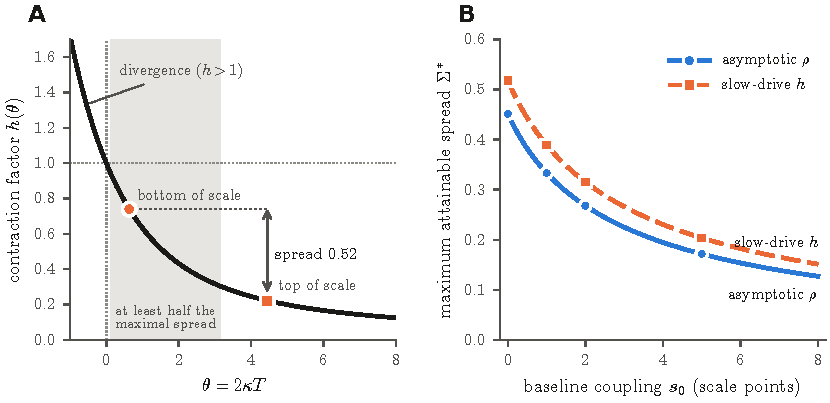
\includegraphics[width=\textwidth]{fig1.pdf}
\end{figure}

\noindent\textbf{Figure 1}\\
\emph{The measurable observable and the ceiling on its contrast}

\begingroup\singlespacing
\noindent\emph{Note.} (A) The contraction factor $h(\theta)=(1-e^{-\theta})/\theta$, the
ratio of the coupled to the uncoupled intake gap at the end of a meal, extended to
$\theta<0$ (divergence, $h>1$). Points mark the ends of a seven-point closeness
scale positioned to maximise their separation; the shaded band is the range of
$\theta$ at the bottom of the scale over which at least half the maximal spread is
retained, ignoring noise. (B) Maximum attainable spread across the scale as a
function of the baseline coupling $s_0$, for the asymptotic factor and for $h$.
Points correspond to the rows of Table~1.\par
\endgroup

\newpage

\begin{figure}[h]
\centering
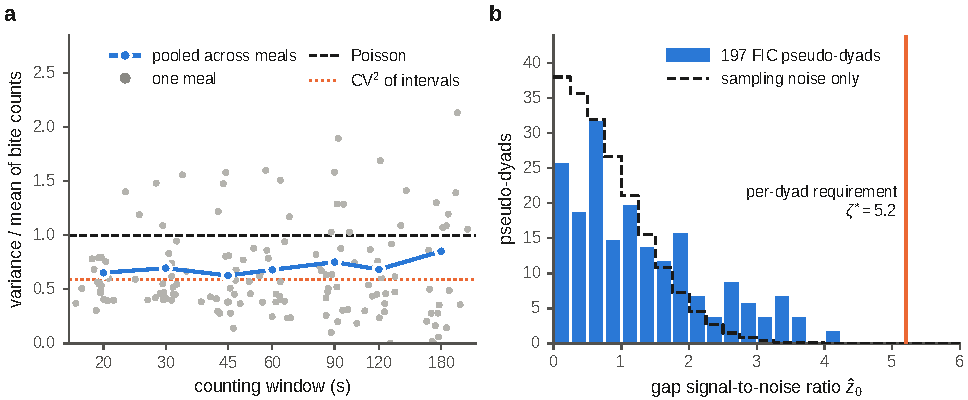
\includegraphics[width=\textwidth]{fig2.pdf}
\end{figure}

\noindent\textbf{Figure 2}\\
\emph{Bite counts are under-dispersed, and no pseudo-dyad reaches the per-dyad requirement}

\begingroup\singlespacing
\noindent\emph{Note.} (A) Variance-to-mean ratio of bite counts in consecutive windows
within each meal (grey points, one per meal and window) and pooled across meals
(line), against the Poisson value of 1 and the squared coefficient of variation
of inter-bite intervals. (B) Gap signal-to-noise ratio $\hat z_0$ of the 197
FIC pseudo-dyads formed from meals of different people, computed from their observed (noise-inflated) contrasts, against
the distribution expected if meals differed only by sampling noise (dashed) and
the per-dyad requirement $\zeta^\star=5.2$.\par
\endgroup

\newpage

\begin{figure}[h]
\centering
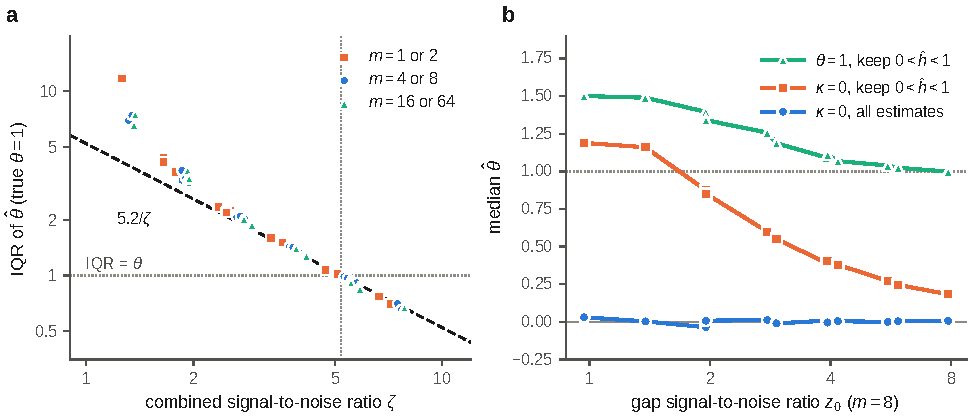
\includegraphics[width=\textwidth]{fig3.pdf}
\end{figure}

\noindent\textbf{Figure 3}\\
\emph{Simulated behaviour of the per-dyad estimator}

\begingroup\singlespacing
\noindent\emph{Note.} (A) Interquartile range of $\hat\theta$ at a true $\theta=1$ against
the combined signal-to-noise ratio $\zeta$, for 72 cells crossing contrast, meal
length and number of solo sessions $m$ (6{,}000 replicates each; cells with an
unbounded IQR omitted). Cells with different $m$ fall on one curve,
$\mathrm{IQR}\approx5.2/\zeta$ (dashed). (B) Median $\hat\theta$ with $m=8$ as a
function of the gap signal-to-noise ratio $z_0$: under no coupling using all
estimates (circles), under no coupling retaining only $0<\hat h<1$ (squares), and
under $\theta=1$ retaining only $0<\hat h<1$ (triangles). The truncated estimator
reports coupling of similar size whether or not any is present.\par
\endgroup

\newpage

\begin{figure}[h]
\centering
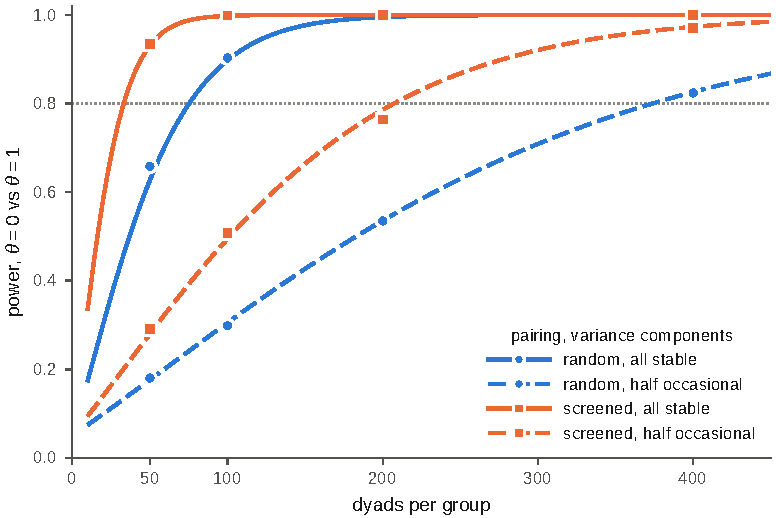
\includegraphics[width=0.62\textwidth]{fig4.pdf}
\end{figure}

\noindent\textbf{Figure 4}\\
\emph{Power of the pooled estimator}

\begingroup\singlespacing
\noindent\emph{Note.} Power to distinguish $\theta=0$ from $\theta=1$ between two groups of
dyads, with 12-minute meals and four solo meals per person. Points: simulation
(1{,}000--2{,}000 replicates); lines: the closed-form variance
\eqref{eq:pooledvar} as implemented in \texttt{couplingdx}. Solid lines assume
between-meal variation in eating rate is entirely stable between people; dashed
lines assign half of it to occasion-to-occasion variation. Screened pairing pairs
opposite terciles of an independent screening meal. The dotted line marks 80\%
power.\par
\endgroup

\end{document}
